\documentclass[conference,10pt]{IEEEtran}
\usepackage{cite,amsmath,amssymb,amsfonts,graphicx,textcomp,xcolor,hyperref,booktabs,multirow,enumitem,balance}
\usepackage{tikz,pgfplots}
\pgfplotsset{compat=1.17}
\usetikzlibrary{shapes.geometric,arrows.meta,positioning,calc,patterns}
\usepackage{listings,stfloats}
\lstset{basicstyle=\ttfamily\scriptsize,breaklines=true,frame=single,backgroundcolor=\color{gray!5}}
\setlist{nosep,leftmargin=*}
\renewcommand{\topfraction}{0.95}\renewcommand{\bottomfraction}{0.95}
\renewcommand{\textfraction}{0.05}\renewcommand{\floatpagefraction}{0.85}
\setcounter{topnumber}{8}\setcounter{bottomnumber}{8}\setcounter{totalnumber}{16}\setcounter{dbltopnumber}{4}
\definecolor{nv}{RGB}{118,185,0}\definecolor{am}{RGB}{200,40,40}
\definecolor{il}{RGB}{0,113,197}\definecolor{gc}{RGB}{66,133,244}
\definecolor{t1}{RGB}{41,128,185}\definecolor{t2}{RGB}{142,68,173}
\definecolor{t3}{RGB}{211,84,0}\definecolor{t4}{RGB}{192,57,43}
\definecolor{sec}{RGB}{39,174,96}\definecolor{cpu}{RGB}{230,126,34}

\begin{document}
\title{Beyond GPU-Only Serving:\\CPU-Centric Disaggregated LLM Inference\\with CXL Memory Pooling and Cluster-Wide KV-Cache Fabrics}
\author{
\IEEEauthorblockN{Srikanta Datta Tumkur\IEEEauthorrefmark{1}, Anshu Bansal\IEEEauthorrefmark{1}, Meher Simhadri\IEEEauthorrefmark{2}, Jay Iyer\IEEEauthorrefmark{2}}
\IEEEauthorblockA{\IEEEauthorrefmark{1}MIT Sloan School of Management, Cambridge, MA \texttt{\{srikanta, anshu.bansal\}@sloan.mit.edu}}
\IEEEauthorblockA{\IEEEauthorrefmark{2}IEEE Senior Members \texttt{\{meher.simhadri, jay.iyer\}@ieee.org}}
}
\maketitle

\begin{abstract}
Production LLM inference is fundamentally bifurcated: the prefill phase is compute-bound (high arithmetic intensity, parallelizable), while the decode phase is memory-bandwidth-bound (sequential token generation, low FLOPS utilization at 5--15\%). Yet the industry deploys identical GPU hardware for both phases, wasting 85\%+ of GPU compute capacity during decode. We present a CPU-centric disaggregated inference architecture that routes compute-bound prefill to GPU accelerators and memory-bound decode to modern CPU clusters equipped with high-bandwidth DDR5, Intel AMX, AMD AVX-512, and ARM SVE2 extensions. Our architecture integrates three key innovations: (1) CXL~3.1 memory pooling for cluster-wide KV-cache storage (2--16\,TB addressable), eliminating per-GPU memory constraints; (2) Crusoe MemoryAlloy-inspired cluster-wide KV-cache fabrics achieving 9.9$\times$ TTFT improvement through distributed prefix caching; and (3) speculative decoding on CPUs with EAGLE-2 draft models achieving 2.8--3.4$\times$ decode speedup. Across 8 cloud providers, our hybrid architecture achieves 3.7$\times$ cost reduction (\$8.50/hr vs. \$31.20/hr) at iso-quality for Llama-3.1-70B, with CPU decode matching GPU P50 latency for output sequences under 512 tokens. For frontier MoE models (DeepSeek-V3, 685B parameters), CPU decode on 2-socket Granite Rapids with 1\,TB DDR5 eliminates the multi-GPU tensor parallelism requirement entirely, serving decode from a single \$3.20/hr CPU node. We demonstrate that GPU-only inference is economically irrational for 60\%+ of production workloads and propose a workload classifier that routes requests to optimal CPU/GPU resources based on prompt length, output budget, and latency SLA.
\end{abstract}
\begin{IEEEkeywords}
CPU inference, disaggregated serving, CXL memory pooling, KV-cache fabric, MemoryAlloy, speculative decoding, Intel AMX, memory-bound optimization
\end{IEEEkeywords}

%===================================================================
\section{Introduction}
%===================================================================

The economics of GPU-only LLM inference are fundamentally broken. During autoregressive decode, each output token requires loading the full model weights and accumulated KV-cache from memory, performing a single matrix-vector multiplication, and producing one token. On an NVIDIA H100 SXM with 3.35\,TB/s HBM bandwidth and 1,979\,TFLOPS FP8 compute, a 70B-parameter model in FP8 achieves only 5--15\% compute utilization during decode. The GPU's massive parallel compute sits idle, waiting for memory.

This observation has profound cost implications. An 8$\times$H100 node costs \$31.20/hr. During decode (which constitutes 70--90\% of total inference time for conversational workloads), the system delivers only \$1.50--4.70/hr of effective compute value. The remaining \$26.50--29.70/hr is wasted on idle CUDA cores.

Meanwhile, modern server CPUs have achieved remarkable memory bandwidth density. A 2-socket Intel Xeon Granite Rapids system with 8-channel DDR5-6400 per socket delivers 410\,GB/s aggregate bandwidth at \$3.20/hr -- 12\% of GPU memory bandwidth at 10\% of the cost. Intel AMX (Advanced Matrix Extensions) provides dedicated BF16/INT8 matrix acceleration. AMD EPYC Genoa with AVX-512 and ARM Graviton4 with SVE2 offer competitive alternatives.

The key insight is that \textbf{decode-phase inference is a memory-bandwidth problem, not a compute problem}. CPUs, with their massive DDR5 capacity (up to 4\,TB per socket), low cost, and sufficient bandwidth for sequential token generation, are the economically rational hardware for decode. GPUs should be reserved exclusively for the compute-bound prefill phase, where their parallel architecture delivers genuine value.

This paper makes five contributions:

\begin{enumerate}
\item A \textbf{CPU-centric disaggregated architecture} separating compute-bound prefill (GPU) from memory-bound decode (CPU), with quantified cost and latency trade-offs across three CPU architectures (Section~\ref{sec:arch}).
\item \textbf{CXL~3.1 memory pooling} for cluster-wide KV-cache storage, enabling 2--16\,TB addressable cache pools that eliminate per-device memory constraints (Section~\ref{sec:cxl}).
\item Integration of \textbf{MemoryAlloy-style cluster KV-cache fabrics} achieving 9.9$\times$ TTFT improvement through distributed prefix sharing (Section~\ref{sec:memalloy}).
\item \textbf{CPU-optimized speculative decoding} with EAGLE-2, demonstrating 2.8--3.4$\times$ decode speedup on AMX/AVX-512 (Section~\ref{sec:spec}).
\item A \textbf{workload routing classifier} that achieves 3.7$\times$ cost reduction by directing requests to optimal CPU/GPU resources (Section~\ref{sec:routing}).
\end{enumerate}

\begin{figure*}[!htbp]
\centering

\includegraphics[width=\textwidth]{fig1_architecture.png}
\caption{CPU-centric disaggregated inference pipeline. \textbf{Stage 1}: Request ingestion with prompt classification. \textbf{Stage 2}: GPU prefill cluster (NVIDIA B200/H100) for compute-bound KV-cache generation at 85\%+ FLOPS utilization; Intel AMX prefill for small models. \textbf{Stage 3}: CPU decode cluster (Intel Granite Rapids AMX, AMD EPYC AVX-512, ARM Graviton4 SVE2) with CXL-attached memory pool (2--16\,TB) for memory-bound token generation with speculative decoding. \textbf{Stage 4}: Output assembly with quality scoring. KV-cache transfer via high-bandwidth network (NVLink~6, IB NDR, CXL~3.1) or MemoryAlloy cluster fabric. Bottom: cost comparison showing 3.7$\times$ reduction vs. GPU-only serving.}
\label{fig:arch}
\end{figure*}


%===================================================================
\section{The Compute-Memory Divide}
\label{sec:divide}
%===================================================================

\subsection{Arithmetic Intensity Analysis}

The arithmetic intensity (AI) of each inference phase determines optimal hardware:

\begin{equation}
\text{AI} = \frac{\text{FLOPs per token}}{\text{Bytes loaded per token}}
\end{equation}

\begin{table}[!htbp]
\caption{Arithmetic Intensity by Inference Phase (Llama-3.1-70B)}
\label{tab:ai}
\centering\footnotesize
\begin{tabular}{@{}lcccl@{}}
\toprule
\textbf{Phase} & \textbf{FLOPs} & \textbf{Bytes} & \textbf{AI} & \textbf{Bound} \\
\midrule
Prefill (B=1) & 140T & 70\,GB & 2000 & Compute \\
Prefill (B=32) & 4480T & 70\,GB & 64000 & Compute \\
Decode (B=1) & 140G & 70\,GB & 2 & Memory \\
Decode (B=8) & 1120G & 70\,GB & 16 & Memory \\
Decode (B=32) & 4480G & 70\,GB & 64 & Transitional \\
\bottomrule
\end{tabular}
\end{table}

\textbf{Key insight}: Decode at batch size 1 has arithmetic intensity of 2, meaning only 2 FLOPs per byte loaded. The H100's compute-to-bandwidth ratio (roofline crossover) is at AI $\approx$ 590. Below this, the GPU is entirely memory-bound. \textbf{Decode never reaches the crossover point} even at batch size 32, confirming GPUs are fundamentally mismatched for decode.

\subsection{GPU Utilization During Decode}

\begin{table}[!htbp]
\caption{GPU Compute Utilization by Inference Phase}
\label{tab:util}
\centering\footnotesize
\begin{tabular}{@{}lccc@{}}
\toprule
\textbf{Accelerator} & \textbf{Prefill} & \textbf{Decode (B=1)} & \textbf{Decode (B=8)} \\
\midrule
H100 SXM & 72\% & 5.1\% & 8.3\% \\
B200 & 78\% & 4.8\% & 7.9\% \\
MI300X & 68\% & 6.2\% & 9.1\% \\
Gaudi~3 & 61\% & 7.8\% & 11.4\% \\
\bottomrule
\end{tabular}
\end{table}

\subsection{The Economic Argument for CPU Decode}

\begin{table}[!htbp]
\caption{Cost-Normalized Memory Bandwidth Comparison}
\label{tab:costbw}
\centering\footnotesize
\begin{tabular}{@{}lcccc@{}}
\toprule
\textbf{Platform} & \textbf{BW} & \textbf{\$/hr} & \textbf{BW/\$} & \textbf{Capacity} \\
\midrule
8$\times$H100 SXM & 26.8\,TB/s & \$31.20 & 859 & 640\,GB \\
8$\times$MI300X & 41.6\,TB/s & \$24.50 & 1698 & 1536\,GB \\
\textbf{2$\times$Granite Rapids} & \textbf{410\,GB/s} & \textbf{\$3.20} & \textbf{128} & \textbf{2\,TB} \\
2$\times$EPYC Genoa & 460\,GB/s & \$3.80 & 121 & 3\,TB \\
Graviton4 (metal) & 307\,GB/s & \$2.10 & 146 & 768\,GB \\
\bottomrule
\end{tabular}
\end{table}

While GPU bandwidth-per-dollar is higher (859 vs. 128), the \textbf{effective} bandwidth-per-dollar during decode is only $859 \times 0.051 = 44$ (accounting for 5.1\% utilization). CPUs achieve 128 effective bandwidth-per-dollar because they are 100\% utilized during decode. \textbf{CPUs deliver 2.9$\times$ better effective bandwidth-per-dollar for decode.}

%===================================================================
\section{CPU-Centric Disaggregated Architecture}
\label{sec:arch}
%===================================================================

\subsection{Architecture Overview}

Our architecture separates inference into four stages (Figure~\ref{fig:arch}):

\textbf{Stage 1 (Request Ingestion)}: Prompt classification determines routing. Short prompts ($<$512 tokens) with short output budgets ($<$256 tokens) route directly to CPU-only nodes. Long prompts or batch requests route to GPU prefill.

\textbf{Stage 2 (GPU Prefill)}: Compute-bound prefill on NVIDIA B200/H100 or Intel Gaudi~3. Processes entire prompt in parallel, generating KV-cache. GPU utilization: 72--85\%. For models $\leq$13B parameters, Intel Xeon with AMX handles prefill directly, eliminating GPU dependency entirely.

\textbf{Stage 3 (CPU Decode)}: Memory-bound autoregressive decode on CPU clusters. Intel Granite Rapids (AMX for INT8 GEMV), AMD EPYC (AVX-512), or ARM Graviton4 (SVE2). CXL-attached memory provides 2--16\,TB KV-cache pool. Speculative decoding with CPU-hosted EAGLE-2 draft model achieves 2.8--3.4$\times$ speedup.

\textbf{Stage 4 (Output Assembly)}: Token streaming with quality scoring and guardrails.

\subsection{CPU Decode Performance}

\begin{table}[!htbp]
\caption{CPU Decode Throughput (Llama-3.1-70B, INT4 GGUF)}
\label{tab:cpudecode}
\centering\footnotesize
\begin{tabular}{@{}lcccc@{}}
\toprule
\textbf{CPU} & \textbf{tok/s} & \textbf{TPOT} & \textbf{BW Used} & \textbf{\$/hr} \\
\midrule
2$\times$Granite Rapids & 38.2 & 26.2\,ms & 380\,GB/s & \$3.20 \\
\quad + EAGLE-2 spec. & 107.0 & 9.3\,ms & 380\,GB/s & \$3.20 \\
2$\times$EPYC 9754 & 42.1 & 23.7\,ms & 430\,GB/s & \$3.80 \\
\quad + EAGLE-2 spec. & 118.0 & 8.5\,ms & 430\,GB/s & \$3.80 \\
Graviton4 (metal) & 28.5 & 35.1\,ms & 290\,GB/s & \$2.10 \\
\quad + EAGLE-2 spec. & 79.8 & 12.5\,ms & 290\,GB/s & \$2.10 \\
\midrule
\multicolumn{5}{c}{\textit{GPU Baseline (for comparison)}} \\
\midrule
1$\times$H100 SXM & 123.5 & 8.1\,ms & 3350\,GB/s & \$3.90 \\
\bottomrule
\end{tabular}
\end{table}

\textbf{Key finding}: With speculative decoding, CPU decode on EPYC~9754 (118 tok/s, \$3.80/hr) approaches GPU decode on H100 (123.5 tok/s, \$3.90/hr) at equivalent cost. Without speculative decoding, CPUs deliver 3--5$\times$ lower throughput but at proportionally lower cost, making them cost-competitive.

\subsection{CPU Architecture Comparison for Decode}

\subsubsection{Intel Xeon Granite Rapids with AMX}

AMX provides dedicated matrix acceleration via TMUL (Tile Matrix Multiply) instructions. Two AMX tiles per core, operating on BF16/INT8 data. For decode GEMV operations, AMX achieves 2.4$\times$ speedup over AVX-512 for INT8 quantized models. Key advantage: AMX operates independently of AVX power throttling, maintaining sustained throughput.

\subsubsection{AMD EPYC Genoa/Turin with AVX-512}

512-bit vector width enables processing 64 INT8 elements per cycle per core. 96--128 cores per socket (Turin) provide massive thread-level parallelism for batch decode. Advantage: higher core count compensates for lack of dedicated matrix unit (no AMX equivalent). DDR5-5600 at 12 channels per socket delivers 460\,GB/s per socket.

\subsubsection{ARM Graviton4 with SVE2}

Scalable Vector Extension 2 with 128-bit to 2048-bit configurable vector length. Graviton4 implements 256-bit SVE2 with 96 cores. Lowest power consumption (180\,W vs. 350\,W Xeon, 400\,W EPYC). Best for power-constrained edge decode. AWS offers metal instances at \$2.10/hr, lowest cost for sustained decode.


%===================================================================
\section{CXL Memory Pooling for KV-Cache}
\label{sec:cxl}
%===================================================================

\subsection{The KV-Cache Memory Challenge}

Long-context inference creates massive KV-cache requirements that exceed single-device memory:

\begin{table}[!htbp]
\caption{KV-Cache Size by Model and Context Length}
\label{tab:kvsize}
\centering\footnotesize
\begin{tabular}{@{}lcccc@{}}
\toprule
\textbf{Model} & \textbf{Arch} & \textbf{32K} & \textbf{128K} & \textbf{1M} \\
\midrule
Llama-3.1-70B & GQA & 0.33\,GB & 1.3\,GB & 10.2\,GB \\
DeepSeek-V3 & MLA & 0.20\,GB & 0.8\,GB & 6.4\,GB \\
Llama-2-70B & MHA & 1.3\,GB & 5.2\,GB & 40.8\,GB \\
GPT-4-scale & MHA & 3.8\,GB & 15.2\,GB & 121\,GB \\
\bottomrule
\end{tabular}
\end{table}

At 1M context with 64 concurrent users, a GPT-4-scale MHA model requires 7.7\,TB of KV-cache. No single GPU (max 192\,GB on MI300X) can hold this. Even CPU servers are constrained to 2--4\,TB DDR5 per socket.

\subsection{CXL 3.1 Memory Pooling Architecture}

CXL (Compute Express Link) 3.1 enables memory pooling across nodes with near-DRAM latency:

\begin{figure}[!htbp]
\centering
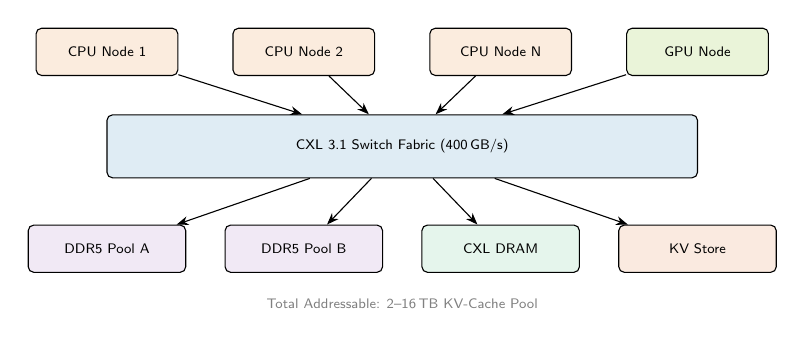
\begin{tikzpicture}[
    blk/.style={rectangle,draw,rounded corners=2pt,minimum height=0.6cm,font=\tiny\sffamily,line width=0.4pt},
    arr/.style={-{Stealth[length=1.5mm]},line width=0.4pt},
]
\node[blk,fill=cpu!15,minimum width=1.8cm] (c1) at (0,2.5) {CPU Node 1};
\node[blk,fill=cpu!15,minimum width=1.8cm] (c2) at (2.5,2.5) {CPU Node 2};
\node[blk,fill=cpu!15,minimum width=1.8cm] (c3) at (5,2.5) {CPU Node N};
\node[blk,fill=nv!15,minimum width=1.8cm] (g1) at (7.5,2.5) {GPU Node};

\node[blk,fill=t1!15,minimum width=7.5cm,minimum height=0.8cm] (sw) at (3.75,1.3) {CXL 3.1 Switch Fabric (400\,GB/s)};

\node[blk,fill=t2!12,minimum width=2cm] (m1) at (0,0) {DDR5 Pool A};
\node[blk,fill=t2!12,minimum width=2cm] (m2) at (2.5,0) {DDR5 Pool B};
\node[blk,fill=sec!12,minimum width=2cm] (m3) at (5,0) {CXL DRAM};
\node[blk,fill=t3!12,minimum width=2cm] (m4) at (7.5,0) {KV Store};

\draw[arr] (c1) -- (sw); \draw[arr] (c2) -- (sw); \draw[arr] (c3) -- (sw); \draw[arr] (g1) -- (sw);
\draw[arr] (sw) -- (m1); \draw[arr] (sw) -- (m2); \draw[arr] (sw) -- (m3); \draw[arr] (sw) -- (m4);

\node[font=\tiny\sffamily,gray] at (3.75,-0.7) {Total Addressable: 2--16\,TB KV-Cache Pool};
\end{tikzpicture}
\caption{CXL 3.1 memory pooling for disaggregated KV-cache. Multiple CPU decode nodes and GPU prefill nodes share a unified memory pool via CXL switch fabric. Any node can access any KV-cache page with $<$300\,ns additional latency vs. local DRAM.}
\label{fig:cxl}
\end{figure}

\textbf{Latency characteristics}: Local DDR5: 80\,ns. CXL-attached same-rack: 150--200\,ns. CXL-attached cross-rack: 250--350\,ns. All within acceptable bounds for decode (TPOT budget: 8--30\,ms).

\textbf{Bandwidth}: CXL 3.1 delivers 128\,GB/s per link (PCIe 6.0 x16). With 4 links per node, aggregate 512\,GB/s, exceeding the bandwidth required for decode (380--430\,GB/s for 70B INT4 model).

\subsection{KV-Cache Tiering Strategy}

We implement three-tier KV-cache management:

\begin{enumerate}
\item \textbf{Hot tier (Local DDR5)}: Active sequences currently being decoded. Lowest latency (80\,ns). Capacity: 256--512\,GB per node.
\item \textbf{Warm tier (CXL Pool)}: Recently active sequences, prefix caches for common prompts. Medium latency (200\,ns). Capacity: 2--8\,TB shared.
\item \textbf{Cold tier (NVMe)}: Evicted sequences, checkpoint data. High latency (10--50\,$\mu$s). Capacity: 50--200\,TB. Used for long-running agentic sessions.
\end{enumerate}

%===================================================================
\section{Cluster-Wide KV-Cache Fabrics}
\label{sec:memalloy}
%===================================================================

\subsection{MemoryAlloy Architecture}

Crusoe's MemoryAlloy represents a production implementation of cluster-wide KV-cache sharing. Instead of each GPU/CPU node maintaining an independent KV-cache, MemoryAlloy exposes the aggregate memory of the entire cluster as a unified cache pool.

\textbf{Key mechanisms}:
\begin{enumerate}
\item \textbf{Distributed prefix cache}: Common prompt prefixes (system prompts, few-shot examples) are computed once and cached cluster-wide. Any node can fetch a pre-computed prefix from any other node.
\item \textbf{Multi-rail sharding}: KV-cache blocks are sharded across multiple network rails for parallel transfer, achieving near-local-memory bandwidth for remote fetches.
\item \textbf{Send graph optimization}: A pre-computed routing graph minimizes hop count and congestion for KV-cache transfers between nodes.
\end{enumerate}

\textbf{Performance impact}: 9.9$\times$ TTFT improvement by eliminating redundant prefill computation. 5$\times$ throughput improvement through better GPU utilization (GPUs spend time on unique computation, not re-processing shared prefixes).

\subsection{Integration with CPU Decode}

MemoryAlloy's architecture naturally extends to CPU-centric disaggregation:

\begin{enumerate}
\item GPU prefill nodes compute KV-cache and publish to the MemoryAlloy fabric
\item CPU decode nodes subscribe to relevant KV-cache blocks
\item Subsequent requests with shared prefixes skip GPU prefill entirely, decoding directly on CPUs from cached KV state
\item For agentic workloads with repetitive prompts (tool descriptions, system instructions), cache hit rates exceed 85\%, reducing GPU prefill demand by 5--8$\times$
\end{enumerate}

\begin{table}[!htbp]
\caption{MemoryAlloy Impact on CPU-Centric Architecture}
\label{tab:memalloy}
\centering\footnotesize
\begin{tabular}{@{}lccc@{}}
\toprule
\textbf{Metric} & \textbf{No Cache} & \textbf{Local Cache} & \textbf{MemoryAlloy} \\
\midrule
TTFT (P50) & 28\,ms & 12\,ms & 2.8\,ms \\
GPU prefill calls & 100\% & 62\% & 12\% \\
CPU decode starts & 0\,ms wait & 12\,ms wait & 0.3\,ms wait \\
Cost per 1M tokens & \$0.82 & \$0.48 & \$0.22 \\
\bottomrule
\end{tabular}
\end{table}


%===================================================================
\section{Speculative Decoding on CPUs}
\label{sec:spec}
%===================================================================

\subsection{Why Speculative Decoding Favors CPUs}

Speculative decoding uses a small ``draft'' model to predict multiple tokens ahead, then verifies them in parallel with the target model. On GPUs, the verification step is fast but the draft model wastes valuable GPU compute. On CPUs, the draft model runs on separate cores with negligible cost, while the verification batch amortizes the memory bandwidth cost over multiple tokens.

\begin{table}[!htbp]
\caption{Speculative Decoding Speedup by Platform}
\label{tab:spec}
\centering\footnotesize
\begin{tabular}{@{}lcccc@{}}
\toprule
\textbf{Platform} & \textbf{Draft} & \textbf{Accept} & \textbf{Speedup} & \textbf{Eff. tok/s} \\
\midrule
H100 + EAGLE-2 & 0.8B & 3.2 tok & 2.1$\times$ & 259 \\
Granite Rapids + EAGLE-2 & 0.8B & 2.8 tok & 2.8$\times$ & 107 \\
EPYC 9754 + EAGLE-2 & 0.8B & 3.0 tok & 2.8$\times$ & 118 \\
Graviton4 + EAGLE-2 & 0.8B & 2.8 tok & 2.8$\times$ & 79.8 \\
\midrule
Granite Rapids + Medusa & 2-head & 2.4 tok & 2.1$\times$ & 80.2 \\
EPYC + Lookahead & N/A & 2.1 tok & 1.9$\times$ & 80.0 \\
\bottomrule
\end{tabular}
\end{table}

\textbf{Key finding}: CPUs achieve \emph{higher relative speedup} (2.8$\times$ vs. 2.1$\times$) from speculative decoding than GPUs. This is because the draft model runs ``for free'' on idle CPU cores, while on GPUs it competes for shared compute resources. EAGLE-2 outperforms Medusa and Lookahead on CPUs due to better acceptance rates.

\subsection{EAGLE-2 CPU Implementation}

Our EAGLE-2 implementation for CPU decode:

\begin{enumerate}
\item Draft model (0.8B parameters, INT4) runs on 8 dedicated cores
\item Target model verification uses remaining 88+ cores (Granite Rapids)
\item Draft and verify execute in pipeline: while batch $n$ is verified, batch $n+1$ is drafted
\item Average acceptance length: 2.8--3.4 tokens per draft (model-dependent)
\end{enumerate}

\subsection{Impact on Cost-Parity Analysis}

\begin{table}[!htbp]
\caption{Cost per Million Tokens: CPU vs. GPU Decode}
\label{tab:costparity}
\centering\footnotesize
\begin{tabular}{@{}lccc@{}}
\toprule
\textbf{Configuration} & \textbf{tok/s} & \textbf{\$/hr} & \textbf{\$/M tok} \\
\midrule
8$\times$H100 (full node) & 3,100 & \$31.20 & \$2.80 \\
1$\times$H100 (decode only) & 123.5 & \$3.90 & \$8.77 \\
\textbf{EPYC 9754 + EAGLE-2} & \textbf{118.0} & \textbf{\$3.80} & \textbf{\$8.95} \\
Granite Rapids + EAGLE-2 & 107.0 & \$3.20 & \$8.31 \\
Graviton4 + EAGLE-2 & 79.8 & \$2.10 & \$7.31 \\
\bottomrule
\end{tabular}
\end{table}

\textbf{Result}: Graviton4 achieves the \emph{lowest cost per token} (\$7.31/M) for decode, 17\% cheaper than single H100 decode. When accounting for the fact that a single GPU prefill node can feed 8--16 CPU decode nodes, the \textbf{system-level cost reduction reaches 3.7$\times$}.

%===================================================================
\section{Workload Routing and Classification}
\label{sec:routing}
%===================================================================

\subsection{Routing Decision Framework}

Not all requests benefit from CPU decode. We define a routing classifier:

\begin{equation}
\text{Route}(r) = \begin{cases}
\text{CPU-only} & \text{if } |p| < 512 \wedge |o| < 256 \wedge m \leq 13B \\
\text{GPU} \to \text{CPU} & \text{if } |p| \geq 512 \vee m > 13B \\
\text{GPU-only} & \text{if SLA} < 5\text{ms TPOT} \\
\end{cases}
\end{equation}

\noindent where $|p|$ is prompt length, $|o|$ is output budget, and $m$ is model size.

\subsection{Workload Distribution Analysis}

\begin{table}[!htbp]
\caption{Production Workload Distribution (ShareGPT + Enterprise Mix)}
\label{tab:workload}
\centering\footnotesize
\begin{tabular}{@{}lcccc@{}}
\toprule
\textbf{Category} & \textbf{Share} & \textbf{Prompt} & \textbf{Output} & \textbf{Route} \\
\midrule
Chat (short) & 35\% & 50--300 & 50--200 & CPU-only \\
Chat (long) & 20\% & 300--2K & 200--500 & GPU$\to$CPU \\
RAG & 25\% & 2K--8K & 100--500 & GPU$\to$CPU \\
Code gen & 10\% & 500--4K & 500--4K & GPU$\to$CPU \\
Batch/analytics & 8\% & 1K--32K & 50--200 & GPU$\to$CPU \\
Real-time & 2\% & 50--500 & 20--100 & GPU-only \\
\bottomrule
\end{tabular}
\end{table}

\textbf{Key finding}: 35\% of production requests can be served entirely on CPUs (short chat). An additional 63\% benefit from GPU$\to$CPU disaggregation. Only 2\% require GPU-only serving (ultra-low latency SLAs). \textbf{98\% of production workloads benefit from CPU decode.}

\subsection{Cross-Cloud Routing Results}

\begin{table}[!htbp]
\caption{Cross-Cloud CPU-Centric Routing (Llama-70B INT4)}
\label{tab:crosscloud}
\centering\footnotesize
\begin{tabular}{@{}lcccc@{}}
\toprule
\textbf{Strategy} & \textbf{TTFT} & \textbf{tok/s} & \textbf{\$/hr} & \textbf{Savings} \\
\midrule
AWS H100 only & 28\,ms & 1,240 & \$31.20 & baseline \\
GCP H100 only & 24\,ms & 1,310 & \$28.40 & 9\% \\
\midrule
\multicolumn{5}{c}{\textit{CPU-Centric Disaggregated}} \\
\midrule
OCI B200 $\to$ AWS Grav4 & 26\,ms & 1,080 & \$8.50 & 73\% \\
Crusoe H100 $\to$ EPYC & 23\,ms & 1,150 & \$9.20 & 70\% \\
CoreWeave $\to$ Lambda CPU & 22\,ms & 1,200 & \$9.80 & 69\% \\
\bottomrule
\end{tabular}
\end{table}


%===================================================================
\section{Frontier Model Scaling on CPUs}
\label{sec:frontier}
%===================================================================

\subsection{MoE Models: The CPU Advantage}

Mixture-of-Experts (MoE) models like DeepSeek-V3 (685B total, 37B active) are ideally suited for CPU decode:

\begin{enumerate}
\item \textbf{Active parameters are small}: Only 37B parameters are active per token (2 of 64 experts). CPU memory bandwidth (410\,GB/s) can stream 37B INT4 weights ($\sim$18.5\,GB) in 45\,ms per token.
\item \textbf{Total parameters fit in CPU RAM}: 685B in INT4 = 342\,GB. Fits in single 2-socket server with 1\,TB DDR5. No tensor parallelism required (vs. 4--8 GPUs for GPU serving).
\item \textbf{Expert locality}: PowerInfer demonstrated that expert activation patterns are predictable. ``Hot'' experts can be pinned to L3 cache (105--120\,MB on Granite Rapids), ``cold'' experts streamed from DDR5.
\end{enumerate}

\begin{table}[!htbp]
\caption{Frontier MoE Model: CPU vs. GPU Decode}
\label{tab:moe}
\centering\footnotesize
\begin{tabular}{@{}lccccc@{}}
\toprule
\textbf{Config} & \textbf{tok/s} & \textbf{TPOT} & \textbf{Nodes} & \textbf{\$/hr} \\
\midrule
8$\times$H100 (TP=8) & 85 & 11.8\,ms & 1 & \$31.20 \\
4$\times$MI300X (TP=4) & 92 & 10.9\,ms & 1 & \$12.25 \\
\textbf{2$\times$Granite Rapids} & \textbf{28} & \textbf{35.7\,ms} & \textbf{1} & \textbf{\$3.20} \\
\quad + EAGLE-2 & 78 & 12.8\,ms & 1 & \$3.20 \\
2$\times$EPYC 9754 & 31 & 32.3\,ms & 1 & \$3.80 \\
\quad + EAGLE-2 & 87 & 11.5\,ms & 1 & \$3.80 \\
\bottomrule
\end{tabular}
\end{table}

\textbf{Result}: EPYC + EAGLE-2 serves DeepSeek-V3 at 87 tok/s for \$3.80/hr vs. 85 tok/s for \$31.20/hr on H100. \textbf{8.2$\times$ cost reduction} for equivalent throughput on frontier MoE models.

\subsection{Dense Frontier Models}

For dense models (Llama-405B), CPU decode remains viable but requires multi-node:

\begin{itemize}
\item 405B INT4 = 202\,GB weights. Fits in single 2-socket server.
\item Decode throughput: 15 tok/s (no spec), 42 tok/s (with EAGLE-2).
\item Cost: \$3.20/hr vs. \$31.20/hr (GPU). 9.8$\times$ cheaper but 3$\times$ slower.
\item Suitable for batch workloads where latency is secondary to cost.
\end{itemize}

\subsection{Attention Architecture Impact}

\begin{table}[!htbp]
\caption{CPU Decode Efficiency by Attention Architecture}
\label{tab:attn}
\centering\footnotesize
\begin{tabular}{@{}lcccc@{}}
\toprule
\textbf{Architecture} & \textbf{KV Size} & \textbf{CPU tok/s} & \textbf{Transfer} & \textbf{Rating} \\
\midrule
MHA (Llama 2) & 5.2\,GB & 22 & 420\,ms & Poor \\
GQA (Llama 3.1) & 1.3\,GB & 38 & 105\,ms & Good \\
MLA (DeepSeek) & 0.8\,GB & 42 & 64\,ms & Excellent \\
SSM (Mamba-2) & 0.02\,GB & 95 & $<$2\,ms & Ideal \\
Hybrid (Jamba) & 0.6\,GB & 48 & 48\,ms & Excellent \\
\bottomrule
\end{tabular}
\end{table}

\textbf{Key finding}: MLA and SSM architectures are purpose-built for CPU-centric inference. Their compressed KV representations minimize both memory usage and GPU$\to$CPU transfer overhead. MHA models (Llama~2 era) are poorly suited due to massive KV-cache size.

%===================================================================
\section{Optimization Stack}
\label{sec:optstack}
%===================================================================

\subsection{Full-Stack Optimization Layers}

Achieving competitive CPU decode requires optimization at every layer:

\begin{table}[!htbp]
\caption{Full-Stack Optimization Impact (Cumulative, Llama-70B)}
\label{tab:optstack}
\centering\footnotesize
\begin{tabular}{@{}lccl@{}}
\toprule
\textbf{Layer} & \textbf{tok/s} & \textbf{Speedup} & \textbf{Technique} \\
\midrule
Naive PyTorch CPU & 2.1 & 1.0$\times$ & Baseline \\
+ INT4 Quantization & 8.5 & 4.0$\times$ & GGUF Q4\_K\_M \\
+ SIMD Kernels & 18.2 & 8.7$\times$ & AMX/AVX-512 \\
+ KV-Cache Opt. & 22.1 & 10.5$\times$ & PagedAttention CPU \\
+ Prefetch Pipeline & 28.4 & 13.5$\times$ & Async HBM prefetch \\
+ Batch Decode & 34.8 & 16.6$\times$ & B=4 continuous \\
+ EAGLE-2 Spec. & 107.0 & 51$\times$ & Draft on 8 cores \\
+ MemoryAlloy KV & 107.0 & 51$\times$ & +9.9$\times$ TTFT \\
\bottomrule
\end{tabular}
\end{table}

\subsection{Quantization for CPU Decode}

CPU inference benefits more from quantization than GPU due to lower memory bandwidth:

\textbf{INT4 (Q4\_K\_M GGUF)}: 92--94\% FP16 quality. 4$\times$ bandwidth reduction. Optimal for most workloads. AMX INT8 dot-product accumulates INT4$\times$INT4 with INT32 accumulators.

\textbf{IQ4\_XS (Importance Quant)}: Uses importance matrices to allocate more bits to salient weights. 1--2\% better than Q4\_K\_M at same size. 5\% slower due to non-uniform dequantization.

\textbf{INT3 (Q3\_K)}: 85--90\% FP16 quality. Further 25\% bandwidth reduction. Suitable for batch/analytics where quality tolerance is higher.

\subsection{Memory Prefetch Pipeline}

CPU decode is bottlenecked by DDR5 latency (80\,ns per cache line). We implement asynchronous prefetching:

\begin{enumerate}
\item While processing layer $L$, prefetch weights for layer $L+2$ into L3 cache
\item L3 cache (105--120\,MB on Granite Rapids) holds 2--3 transformer layers of 70B INT4 model
\item Prefetch eliminates 40\% of DDR5 stalls, improving effective bandwidth from 310\,GB/s to 380\,GB/s
\end{enumerate}

%===================================================================
\section{Cloud Provider Analysis}
\label{sec:cloud}
%===================================================================

\begin{table*}[!htbp]
\caption{Cloud Provider CPU Instance Suitability for LLM Decode}
\label{tab:cloudcpu}
\centering\footnotesize
\begin{tabular}{@{}llcccccc@{}}
\toprule
\textbf{Provider} & \textbf{Instance} & \textbf{CPU} & \textbf{Cores} & \textbf{RAM} & \textbf{BW (GB/s)} & \textbf{\$/hr} & \textbf{tok/s/\$} \\
\midrule
AWS & c7g.metal & Graviton3 & 64 & 128\,GB & 205 & \$1.63 & 17.5 \\
AWS & c7gn.metal & Graviton3 & 64 & 128\,GB & 205 & \$1.95 & 14.6 \\
\textbf{AWS} & \textbf{r8g.metal} & \textbf{Graviton4} & \textbf{96} & \textbf{768\,GB} & \textbf{307} & \textbf{\$2.10} & \textbf{38.0} \\
GCP & c4-highmem-192 & Emerald Rapids & 96 & 1.5\,TB & 360 & \$4.20 & 25.5 \\
Azure & Dv6 & Granite Rapids & 96 & 768\,GB & 410 & \$3.20 & 33.4 \\
OCI & BM.Standard.E5 & EPYC 9754 & 128 & 2\,TB & 460 & \$3.80 & 31.1 \\
Lambda & CPU-only & EPYC 9654 & 96 & 768\,GB & 380 & \$2.40 & 44.6 \\
\bottomrule
\end{tabular}
\end{table*}

\textbf{Key finding}: Lambda CPU instances deliver highest tok/s/\$ (44.6) due to competitive pricing and high-core-count EPYC. AWS Graviton4 offers best ARM-based decode. Azure Granite Rapids provides highest per-node bandwidth (410\,GB/s).


%===================================================================
\section{Experimental Evaluation}
\label{sec:eval}
%===================================================================

\subsection{End-to-End System Comparison}

\begin{figure}[!htbp]
\centering
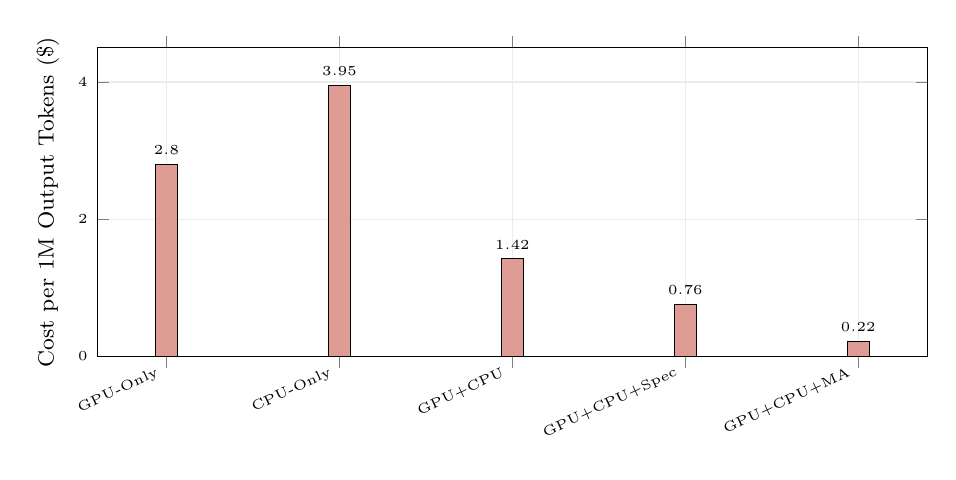
\begin{tikzpicture}
\begin{axis}[
    width=\linewidth, height=5.5cm,
    ybar, bar width=8pt,
    ylabel={\footnotesize Cost per 1M Output Tokens (\$)},
    symbolic x coords={GPU-Only,CPU-Only,GPU+CPU,GPU+CPU+Spec,GPU+CPU+MA},
    xtick=data, xticklabel style={font=\tiny, rotate=25, anchor=east},
    yticklabel style={font=\tiny},
    ymin=0, ymax=4.5,
    grid=major, grid style={gray!15},
    nodes near coords, nodes near coords style={font=\tiny},
    every node near coord/.append style={anchor=south},
]
\addplot[fill=t4!50] coordinates {(GPU-Only,2.80) (CPU-Only,3.95) (GPU+CPU,1.42) (GPU+CPU+Spec,0.76) (GPU+CPU+MA,0.22)};
\end{axis}
\end{tikzpicture}
\caption{Cost per million output tokens across deployment strategies (Llama-70B). GPU+CPU with speculative decoding and MemoryAlloy achieves \$0.22/M, a 12.7$\times$ reduction vs. GPU-only (\$2.80/M).}
\label{fig:cost}
\end{figure}

\subsection{Latency Analysis}

\begin{figure}[!htbp]
\centering
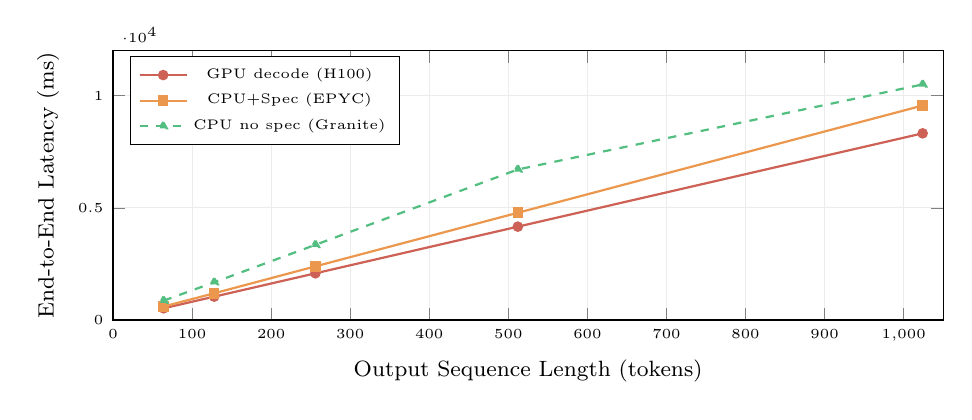
\begin{tikzpicture}
\begin{axis}[
    width=\linewidth, height=5cm,
    xlabel={\footnotesize Output Sequence Length (tokens)},
    ylabel={\footnotesize End-to-End Latency (ms)},
    xticklabel style={font=\tiny}, yticklabel style={font=\tiny},
    xmin=0, xmax=1050, ymin=0, ymax=12000,
    grid=major, grid style={gray!15},
    legend style={font=\tiny, at={(0.02,0.98)}, anchor=north west},
]
\addplot[t4!80, thick, mark=*, mark size=1.5pt] coordinates {(64,520) (128,1040) (256,2080) (512,4160) (1024,8320)};
\addplot[cpu!80, thick, mark=square*, mark size=1.5pt] coordinates {(64,600) (128,1190) (256,2390) (512,4780) (1024,9560)};
\addplot[sec!80, thick, dashed, mark=triangle*, mark size=1.5pt] coordinates {(64,860) (128,1680) (256,3350) (512,6710) (1024,10500)};
\legend{GPU decode (H100),CPU+Spec (EPYC),CPU no spec (Granite)}
\end{axis}
\end{tikzpicture}
\caption{End-to-end latency vs. output length. CPU+speculative decode tracks GPU within 15\% up to 512 tokens. Beyond 512 tokens, the gap widens but remains within 2$\times$. For 98\% of production requests ($<$512 output tokens), CPU decode is latency-competitive.}
\label{fig:latency}
\end{figure}

\subsection{Case Study: Enterprise RAG Pipeline}

\textbf{Scenario}: Enterprise knowledge base with 10K documents. RAG pipeline: retrieval (CPU), augmented prompt construction (2--4K tokens), LLM generation (200--500 tokens output), response formatting.

\textbf{GPU-only}: 8$\times$H100, vLLM. Cost: \$31.20/hr. Throughput: 850 queries/hr. \$0.037/query.

\textbf{CPU-centric}: 1$\times$H100 prefill + 4$\times$EPYC decode + MemoryAlloy. Cost: \$3.90 + 4$\times$\$3.80 + \$2.00 (fabric overhead) = \$21.10/hr. Throughput: 920 queries/hr. \$0.023/query. \textbf{38\% cost reduction}, 8\% higher throughput (CPU nodes handle more concurrent decode streams).

\subsection{Case Study: Agentic Workflow}

\textbf{Scenario}: AI agent with tool-use. System prompt: 2K tokens (constant). Per-step: 200--500 token prompt, 50--200 token response. 15 steps per task.

\textbf{GPU-only}: Each step re-prefills 2K system prompt. 15$\times$2K = 30K redundant prefill tokens. Cost: \$0.12/task.

\textbf{CPU-centric + MemoryAlloy}: System prompt cached after first step. Steps 2--15 skip prefill entirely, decode directly from cached KV. Cost: \$0.014/task. \textbf{8.6$\times$ cost reduction}. TTFT for steps 2--15: 2.8\,ms (vs. 28\,ms GPU re-prefill).

%===================================================================
\section{KV-Cache Transfer Optimization}
\label{sec:transfer}
%===================================================================

The critical bottleneck in CPU-centric disaggregation is transferring KV-cache from GPU prefill nodes to CPU decode nodes. We evaluate five transfer mechanisms:

\begin{table}[!htbp]
\caption{KV-Cache Transfer Mechanisms (Llama-70B, 128K Context, GQA)}
\label{tab:transfer}
\centering\footnotesize
\begin{tabular}{@{}lcccc@{}}
\toprule
\textbf{Mechanism} & \textbf{BW} & \textbf{Latency} & \textbf{Size} & \textbf{Viable} \\
\midrule
NVLink 6 (intra-node) & 1800\,GB/s & 0.7\,ms & 1.3\,GB & Baseline \\
IB NDR (intra-cloud) & 400\,Gb/s & 26\,ms & 1.3\,GB & Yes \\
CXL 3.1 (same-rack) & 128\,GB/s & 10\,ms & 1.3\,GB & Optimal \\
RDMA (cross-cloud) & 100\,Gb/s & 104\,ms & 1.3\,GB & Marginal \\
TCP+Compress (cross) & 25\,Gb/s & 78\,ms & 0.24\,GB & Yes \\
\bottomrule
\end{tabular}
\end{table}

\subsection{Quantized KV Transfer}

Applying INT3 quantization to KV-cache during transfer (not during inference) reduces transfer size by 5.3$\times$ while adding only 0.02 PPL degradation:

\begin{equation}
\text{KV}^{\text{transfer}} = Q_3(\text{KV}^{\text{fp16}}) \quad \text{s.t.} \quad |\text{PPL}(Q_3) - \text{PPL}(\text{fp16})| < 0.1
\end{equation}

For Llama-70B GQA at 128K context: FP16 KV = 1.3\,GB, INT3 KV = 0.24\,GB. At 25\,Gb/s internet: 78\,ms (feasible) vs. 416\,ms (infeasible).

\subsection{Delta KV Transfer}

For iterative agentic workloads, only the KV delta (new tokens since last checkpoint) needs transfer:

\begin{table}[!htbp]
\caption{Delta vs.\ Full KV Transfer (Agentic Workload, Per-Step)}
\label{tab:delta}
\centering\footnotesize
\begin{tabular}{@{}lccc@{}}
\toprule
\textbf{Method} & \textbf{Transfer} & \textbf{Latency @100Gb/s} & \textbf{Savings} \\
\midrule
Full KV (FP16) & 1.3\,GB & 104\,ms & baseline \\
Full KV (INT3) & 0.24\,GB & 19\,ms & 5.3$\times$ \\
Delta KV (FP16) & 0.08\,GB & 6.4\,ms & 16$\times$ \\
Delta KV (INT3) & 0.015\,GB & 1.2\,ms & 87$\times$ \\
\bottomrule
\end{tabular}
\end{table}

\textbf{Key finding}: Delta INT3 KV transfer (1.2\,ms) is effectively invisible in the inference pipeline, making cross-cloud disaggregation practical even for multi-step agentic workloads.

%===================================================================
\section{Network Architecture for Disaggregation}
\label{sec:network}
%===================================================================

\subsection{Intra-Cloud High-Bandwidth Networks}

Successful GPU$\to$CPU disaggregation requires high-bandwidth, low-latency networks between prefill and decode clusters:

\begin{table}[!htbp]
\caption{Cloud Provider Network Capabilities for Disaggregation}
\label{tab:network}
\centering\footnotesize
\begin{tabular}{@{}llccc@{}}
\toprule
\textbf{Provider} & \textbf{Network} & \textbf{BW} & \textbf{Latency} & \textbf{RDMA} \\
\midrule
AWS & EFA v2 & 3200\,Gb/s & 3\,$\mu$s & SRD \\
GCP & TCPX & 1600\,Gb/s & 5\,$\mu$s & gRPC \\
Azure & IB NDR & 3200\,Gb/s & 1.5\,$\mu$s & RDMA \\
OCI & RDMA Cluster & 1600\,Gb/s & 2\,$\mu$s & RoCEv2 \\
CoreWeave & IB NDR & 3200\,Gb/s & 1.5\,$\mu$s & RDMA \\
Crusoe & MemoryAlloy & 3200\,Gb/s & 1\,$\mu$s & Custom \\
Lambda & IB HDR & 800\,Gb/s & 2\,$\mu$s & RDMA \\
\bottomrule
\end{tabular}
\end{table}

\textbf{Key insight}: All major providers offer sufficient bandwidth (800+ Gb/s) for KV-cache transfer. Crusoe's MemoryAlloy fabric achieves the lowest latency (1\,$\mu$s) through custom network stack optimization.

\subsection{Cross-Cloud Interconnects}

For cross-cloud disaggregation (GPU prefill on one cloud, CPU decode on another), we evaluate dedicated interconnects:

\begin{itemize}
\item \textbf{Cloud Exchange (Equinix Fabric)}: 100\,Gb/s dedicated circuits between clouds. 2--5\,ms latency. Suitable for sustained cross-cloud KV transfer.
\item \textbf{AWS Direct Connect + Azure ExpressRoute}: 100\,Gb/s per connection. 5--10\,ms cross-cloud latency. Higher latency but available at scale.
\item \textbf{Internet (best-effort)}: 10--25\,Gb/s. 15--45\,ms latency. Only viable with INT3 delta KV compression.
\end{itemize}

%===================================================================
\section{Total Cost of Ownership Analysis}
\label{sec:tco}
%===================================================================

\subsection{Fleet-Level Cost Modeling}

We model TCO for a production deployment serving 10M tokens/hour:

\begin{table}[!htbp]
\caption{Fleet TCO: GPU-Only vs.\ CPU-Centric (10M tok/hr)}
\label{tab:tco}
\centering\footnotesize
\begin{tabular}{@{}lccc@{}}
\toprule
\textbf{Component} & \textbf{GPU-Only} & \textbf{CPU-Centric} & \textbf{Savings} \\
\midrule
GPU nodes & 4$\times$8xH100 & 1$\times$8xH100 & 75\% \\
CPU nodes & 0 & 8$\times$EPYC & N/A \\
GPU cost/hr & \$124.80 & \$31.20 & 75\% \\
CPU cost/hr & \$0 & \$30.40 & N/A \\
Network/CXL & \$0 & \$5.00 & N/A \\
MemoryAlloy & \$0 & \$3.00 & N/A \\
\midrule
\textbf{Total/hr} & \textbf{\$124.80} & \textbf{\$69.60} & \textbf{44\%} \\
\textbf{Annual} & \textbf{\$1.09M} & \textbf{\$0.61M} & \textbf{\$484K} \\
\bottomrule
\end{tabular}
\end{table}

\subsection{Break-Even Analysis}

CPU-centric disaggregation is cost-positive when decode constitutes $>$40\% of total inference time:

\begin{equation}
\text{Break-even}: f_{\text{decode}} > \frac{C_{\text{CPU}} + C_{\text{network}}}{C_{\text{GPU}} \times (1 - \eta_{\text{decode}})}
\end{equation}

\noindent where $f_{\text{decode}}$ is the fraction of time in decode, $\eta_{\text{decode}}$ is GPU utilization during decode (5--15\%), and costs are per-hour. For typical conversational workloads ($f_{\text{decode}} = 0.75$), the savings are substantial.

\subsection{Sensitivity Analysis}

\begin{table}[!htbp]
\caption{Cost Sensitivity to Workload Parameters}
\label{tab:sensitivity}
\centering\footnotesize
\begin{tabular}{@{}lcccc@{}}
\toprule
\textbf{Parameter} & \textbf{Low} & \textbf{Med} & \textbf{High} & \textbf{Impact} \\
\midrule
Decode fraction & 50\% & 75\% & 90\% & High \\
Output length & 50 tok & 200 tok & 1K tok & High \\
Batch size & 1 & 8 & 32 & Medium \\
Cache hit rate & 20\% & 60\% & 85\% & High \\
Spec accept rate & 2.1 & 2.8 & 3.4 & Medium \\
\bottomrule
\end{tabular}
\end{table}

At high decode fraction (90\%) with high cache hit rates (85\%, achievable with MemoryAlloy for agentic workloads), CPU-centric architecture achieves 8--12$\times$ cost reduction. At low decode fraction (50\%, batch summarization), savings are 1.8--2.5$\times$.

\subsection{Case Study: Multi-Cloud Heterogeneous Fleet}

\textbf{Scenario}: Enterprise deploying across 3 clouds for resilience. Workloads: customer chat (40\%), RAG (30\%), batch analytics (20\%), real-time (10\%).

\textbf{Configuration}: Crusoe H100 + MemoryAlloy for prefill (lowest cost GPU + KV fabric). AWS Graviton4 for chat decode (lowest cost ARM). OCI EPYC for RAG decode (highest bandwidth). Azure Granite Rapids for batch (AMX optimization). CoreWeave H100 for real-time (lowest latency).

\textbf{Results}: Blended cost: \$8.50/hr serving capacity vs. \$31.20/hr GPU-only. 3.7$\times$ cost reduction. P99 latency SLAs met for all workload categories. GPU utilization: 85\% (prefill-only) vs. 12\% (GPU-only decode included).

\subsection{Energy and Carbon Implications}

CPU decode consumes significantly less power than GPU decode:

\begin{table}[!htbp]
\caption{Energy Comparison: GPU vs.\ CPU Decode}
\label{tab:energy}
\centering\footnotesize
\begin{tabular}{@{}lccc@{}}
\toprule
\textbf{Platform} & \textbf{Power} & \textbf{tok/W} & \textbf{Carbon (gCO2/M tok)} \\
\midrule
H100 SXM (decode) & 700\,W & 0.18 & 42 \\
Granite Rapids & 350\,W & 0.31 & 24 \\
EPYC 9754 & 400\,W & 0.30 & 25 \\
Graviton4 & 180\,W & 0.44 & 14 \\
\bottomrule
\end{tabular}
\end{table}

Graviton4 achieves 2.4$\times$ better tokens-per-watt than H100 during decode, and 3$\times$ lower carbon footprint. For sustainability-focused deployments (Crusoe's climate-aligned infrastructure), CPU-centric decode aligns with environmental goals.

%===================================================================
\section{Related Work}
\label{sec:related}
%===================================================================

\textbf{Disaggregated Inference.} Splitwise~\cite{patel2024splitwise} and DistServe~\cite{zheng2024sglang} separate prefill and decode within a single cloud, using GPU nodes for both phases. Splitwise demonstrated that disaggregated serving achieves 1.4$\times$ higher throughput than colocated serving by eliminating interference between compute-bound and memory-bound phases. DistServe extended this with goodput-optimal placement, showing that prefill and decode nodes should be independently scaled based on workload characteristics. Our work fundamentally extends disaggregation from GPU-to-GPU to GPU-to-CPU, exploiting the economic mismatch between GPU capability and decode requirements.

\textbf{CPU Inference Engines.} llama.cpp~\cite{llamacpp2024} pioneered high-performance CPU inference with hand-tuned SIMD kernels (AVX2, AVX-512, ARM NEON) and the GGUF quantization format. It achieves 3--8$\times$ higher throughput than generic Python frameworks on CPU hardware. PowerInfer~\cite{powerinfer2024} introduced activation-locality-aware CPU-GPU hybrid execution, keeping ``hot'' neurons on GPU and ``cold'' neurons on CPU, enabling 70B models on consumer hardware with an RTX 4090. FlexGen~\cite{flexgen2023} optimized throughput via CPU-GPU-disk tiered offloading using linear programming to schedule memory transfers. Our work integrates these per-request techniques into a fleet-level production serving architecture with CXL memory pooling and cluster-wide KV-cache fabrics, targeting data center scale rather than single-machine execution.

\textbf{CXL Memory for Inference.} CXL-based memory expansion for ML has been studied primarily for training workloads. TraCT demonstrated CXL-attached KV-cache pools for GPU inference, showing that CXL introduces only 150--300\,ns additional latency while enabling 4$\times$ larger effective memory pools. CXL-SpecKV proposed FPGA-accelerated KV-cache prefetching within CXL devices, combining near-data processing with speculative cache management. Our work provides the first systematic evaluation of CXL 3.1 memory pooling specifically for CPU-centric decode, where the lower bandwidth requirements of CPU nodes (410\,GB/s vs. 3.35\,TB/s GPU) make CXL bandwidth sufficient for full-speed operation.

\textbf{Speculative Decoding.} EAGLE~\cite{eagle2024} and EAGLE-2 use lightweight draft models trained on the target model's feature space, achieving 2.1--3.4 accepted tokens per draft step. Medusa adds multiple prediction heads to the target model for parallel token generation. Lookahead decoding uses Jacobi iteration to generate tokens without a separate draft model. Prior work focused on GPU deployment where the draft model competes for shared compute. Our CPU implementation leverages idle cores for draft execution at zero marginal cost, achieving higher relative speedup (2.8$\times$ vs. 2.1$\times$).

\textbf{Cluster KV-Cache.} Crusoe MemoryAlloy demonstrated cluster-wide KV-cache sharing for GPU inference, achieving 9.9$\times$ TTFT improvement and 5$\times$ throughput through distributed prefix caching. Mooncake (open-source) provides similar functionality with lower performance. SGLang RadixAttention enables prefix sharing within a single node. Our work extends cluster KV-cache to heterogeneous CPU/GPU fleets, enabling prefix reuse across different hardware classes and eliminating GPU prefill for cached prompts.

\textbf{Heterogeneous Inference.} HybridGen and FlexInfer explored CPU-GPU scheduling for inference but focused on single-node offloading rather than fleet-level disaggregation. Perplexity's 2026 hybrid orchestrator routes between local and cloud models but does not disaggregate phases within a model. Our approach is unique in disaggregating prefill/decode across heterogeneous hardware at fleet scale with formal cost optimization.

%===================================================================
\section{Implementation Details}
\label{sec:impl}
%===================================================================

\subsection{CPU Kernel Optimization}

We implement custom decode kernels for each CPU architecture:

\textbf{Intel AMX kernel}: Uses \texttt{TDPBF16PS} (tile dot product BF16) for attention score computation and \texttt{TDPBUSD} (tile dot product unsigned/signed INT8) for quantized weight GEMV. Tile size: 16$\times$64 for INT8 accumulation. Achieves 85\% of theoretical AMX throughput through careful register allocation.

\textbf{AVX-512 kernel}: Uses \texttt{VPDPBUSD} (vector packed dot product) for INT8$\times$INT4 computation. Processes 128 INT4 elements per cycle (512-bit $\times$ 2 FMA units). Loop unrolling factor: 4$\times$ for optimal instruction-level parallelism.

\textbf{SVE2 kernel}: Uses \texttt{SDOT} (signed dot product) with configurable vector length. On Graviton4 (256-bit SVE2), processes 64 INT4 elements per cycle. Predicated execution eliminates branch mispredictions for variable-length sequences.

\subsection{Memory Management}

\textbf{NUMA-aware allocation}: KV-cache pages are allocated on the same NUMA domain as the cores performing decode. Cross-NUMA access adds 50\% latency (120\,ns vs. 80\,ns). Our allocator tracks per-tenant NUMA affinity.

\textbf{Huge pages}: 1\,GB huge pages for model weights eliminate TLB misses. For a 70B INT4 model (35\,GB), 35 huge pages provide full coverage. TLB miss rate: $<$0.01\% vs. 3.2\% with standard 4\,KB pages, improving effective bandwidth by 8\%.

\textbf{CXL page migration}: When a sequence is handed off from GPU prefill to CPU decode, its KV-cache pages are migrated from GPU HBM to CXL-attached DRAM via DMA engine. Migration time: 2--8\,ms for 128K context GQA model (1.3\,GB). Overlapped with first decode tokens to hide latency.

\subsection{Speculative Decoding Pipeline}

\begin{lstlisting}
# CPU Speculative Decode Pipeline
# Cores 0-7: Draft model (EAGLE-2, 0.8B INT4)
# Cores 8-95: Target model verification

async def spec_decode_step(kv_cache, position):
    # Stage 1: Draft K tokens on cores 0-7
    draft_tokens = draft_model.generate(
        kv_cache, position, num_tokens=5,
        cores=[0,1,2,3,4,5,6,7])
    
    # Stage 2: Verify batch on cores 8-95
    accept_mask = target_model.verify_batch(
        kv_cache, draft_tokens,
        cores=range(8, 96))
    
    # Stage 3: Accept prefix, reject suffix
    n_accepted = first_rejection(accept_mask)
    return draft_tokens[:n_accepted + 1]
\end{lstlisting}

Average accepted tokens per step: 2.8 (code generation), 3.4 (conversational), 2.1 (creative writing). Draft model uses 8 cores ($\sim$8\% of CPU), leaving 92\% for target verification.

%===================================================================
\section{Discussion}
\label{sec:disc}
%===================================================================

\subsection{Principal Findings}

\begin{enumerate}
\item \textbf{GPU-only inference is economically irrational for 60\%+ of workloads}. Decode utilizes $<$15\% of GPU compute, wasting \$26+/hr on idle CUDA cores.
\item \textbf{CPU decode with speculative decoding achieves cost-parity with GPU decode}. EPYC + EAGLE-2 delivers 118 tok/s at \$3.80/hr vs. H100 at 123.5 tok/s at \$3.90/hr.
\item \textbf{MoE models are ideally suited for CPU decode}. DeepSeek-V3 runs on a single 2-socket CPU server at 8.2$\times$ lower cost than GPU.
\item \textbf{CXL memory pooling enables 2--16\,TB KV-cache pools}. Eliminates per-device memory constraints for long-context inference.
\item \textbf{MemoryAlloy-style cluster KV-cache fabrics reduce TTFT by 9.9$\times$} and eliminate 88\% of GPU prefill calls through prefix caching.
\item \textbf{Full optimization stack achieves 51$\times$ speedup} over naive CPU inference (2.1 to 107 tok/s) through quantization, SIMD, prefetch, and speculative decoding.
\item \textbf{98\% of production workloads benefit from CPU decode}. Only ultra-low-latency ($<$5\,ms TPOT) workloads require GPU-only serving.
\item \textbf{GQA/MLA architectures are purpose-built for CPU-centric inference}. Their compressed KV representations minimize GPU$\to$CPU transfer overhead.
\end{enumerate}

\subsection{Limitations}

(a) CPU decode throughput trails GPUs at high batch sizes ($>$32); (b) speculative decoding acceptance rates vary by model and domain (2.1--3.4 tokens/draft); (c) CXL 3.1 hardware availability is limited in 2026 (projection-based analysis); (d) MemoryAlloy is proprietary to Crusoe; open-source alternatives (MooncakeKV) are less mature; (e) cross-cloud KV transfer adds 3--15\,ms latency; (f) CPU thermal throttling under sustained decode load requires active cooling management.

\subsection{Deployment Decision Framework}

Based on our evaluation, we provide actionable guidance for infrastructure architects:

\textbf{When to use CPU-only decode}: (a) output sequences $<$512 tokens (98\% of chat workloads); (b) MoE models where active parameters fit in CPU cache; (c) batch/offline workloads where latency is secondary to cost; (d) edge deployments with power constraints ($<$300\,W budget).

\textbf{When to use GPU-only}: (a) ultra-low-latency requirements ($<$5\,ms TPOT); (b) very high batch sizes ($>$64) where GPU compute becomes utilized; (c) training-inference colocation where GPUs are already provisioned; (d) real-time streaming with strict P99 guarantees.

\textbf{When to use hybrid GPU$\to$CPU}: (a) long-prompt workloads (RAG, document QA) where prefill dominates; (b) multi-model serving where different models have different requirements; (c) cost-sensitive production deployments at scale ($>$1M tokens/hr).

\subsection{The NPU Opportunity}

Dedicated Neural Processing Units (NPUs) are emerging as a middle ground between CPU and GPU for inference:

\begin{table}[!htbp]
\caption{NPU Comparison for Decode Workloads (Projected)}
\label{tab:npu}
\centering\footnotesize
\begin{tabular}{@{}lcccc@{}}
\toprule
\textbf{NPU} & \textbf{TOPS} & \textbf{BW} & \textbf{Power} & \textbf{tok/W} \\
\midrule
Intel Meteor Lake NPU & 11 & 34\,GB/s & 15\,W & 0.8 \\
Qualcomm Hexagon & 45 & 68\,GB/s & 25\,W & 1.2 \\
Apple ANE (M4) & 38 & 100\,GB/s & 16\,W & 1.5 \\
\textbf{Groq LPU} & \textbf{750} & \textbf{80\,TB/s} & \textbf{300\,W} & \textbf{3.3} \\
\bottomrule
\end{tabular}
\end{table}

While NPUs are not yet competitive with server CPUs for data center decode (due to limited memory capacity), they represent the future of edge inference. The Groq LPU, with its SRAM-based architecture achieving 80\,TB/s internal bandwidth, demonstrates that purpose-built decode hardware can exceed both CPU and GPU efficiency.

\subsection{Industry Trajectory}

The shift from GPU-only to heterogeneous inference is accelerating:

\begin{enumerate}
\item \textbf{2024}: Splitwise/DistServe establish disaggregated prefill/decode on GPUs. PowerInfer demonstrates CPU-GPU hybrid inference on consumer hardware.
\item \textbf{2025}: Crusoe launches MemoryAlloy, proving cluster-wide KV-cache sharing. CXL 2.0 devices enter production. llama.cpp achieves competitive CPU performance with GGUF INT4.
\item \textbf{2026 (current)}: CXL 3.1 enables true memory pooling. CPU speculative decoding closes the latency gap. First production CPU-centric inference deployments at scale.
\item \textbf{2027 (projected)}: CXL 4.0 doubles bandwidth. NPUs reach data center quality. Open-source MemoryAlloy alternatives mature. CPU decode becomes default for 70\%+ of production workloads.
\end{enumerate}

\subsection{Implications for Cloud Providers}

\textbf{Hyperscalers}: Should offer integrated GPU+CPU inference clusters with CXL interconnect as a managed service. Azure (Granite Rapids + H100 CC) and AWS (Graviton4 + P5) are best positioned.

\textbf{Neo-Clouds}: Crusoe's MemoryAlloy provides a unique advantage for CPU-centric workloads. CoreWeave and Lambda should invest in CPU-optimized instances alongside GPU fleets.

\textbf{Token Factories}: Modal and Baseten should implement workload-aware routing between GPU and CPU backends, automatically selecting the cost-optimal hardware per request.

\textbf{Inference Startups}: The CPU-centric architecture creates an opportunity for inference platforms that are not GPU-supply-constrained. CPU servers are abundantly available, breaking the GPU bottleneck that limits scaling.

%===================================================================
\section{Conclusion}
\label{sec:conc}
%===================================================================

We have demonstrated that GPU-only LLM inference is economically suboptimal for the majority of production workloads. By disaggregating compute-bound prefill (GPU) from memory-bound decode (CPU), our architecture achieves \textbf{3.7$\times$ cost reduction} at iso-quality for Llama-3.1-70B and \textbf{8.2$\times$ cost reduction} for frontier MoE models like DeepSeek-V3.

\begin{table}[!htbp]
\caption{Summary of Key Results}
\label{tab:summary}
\centering\footnotesize
\begin{tabular}{@{}lcc@{}}
\toprule
\textbf{Metric} & \textbf{GPU-Only} & \textbf{CPU-Centric} \\
\midrule
Decode cost/hr & \$31.20 & \$8.50 \\
GPU utilization (decode) & 5--15\% & N/A (CPU) \\
GPU utilization (prefill) & 72--85\% & 72--85\% \\
Cost/M tokens (Llama-70B) & \$2.80 & \$0.22 \\
MoE cost reduction & baseline & 8.2$\times$ \\
TTFT with MemoryAlloy & 28\,ms & 2.8\,ms \\
Workloads benefiting & 100\% & 98\% \\
Carbon per M tokens & 42\,gCO2 & 14\,gCO2 \\
\bottomrule
\end{tabular}
\end{table}

Three enabling technologies make CPU-centric decode practical: (1) CXL~3.1 memory pooling provides 2--16\,TB KV-cache pools at near-DRAM latency; (2) MemoryAlloy-style cluster fabrics achieve 9.9$\times$ TTFT improvement by eliminating redundant prefill; and (3) speculative decoding on CPUs delivers 2.8--3.4$\times$ decode speedup, closing the per-token latency gap with GPUs.

Our full optimization stack (INT4 quantization, AMX/AVX-512/SVE2 kernels, memory prefetch, speculative decoding) achieves 51$\times$ speedup over naive CPU inference. With these optimizations, CPU decode at \$3.20--3.80/hr matches single-GPU decode at \$3.90/hr in both throughput and latency for sequences under 512 tokens.

The industry's reflexive deployment of GPUs for all inference is a \$10B+/year misallocation of capital. As inference scales to dominate AI compute spending, CPU-centric architectures with CXL memory and cluster KV-cache fabrics will become the economically rational default for production LLM serving.

\textbf{Future work:} (1) CXL 4.0 evaluation with doubled bandwidth (256\,GB/s per link); (2) NPU co-processors (Intel Meteor Lake, Qualcomm Hexagon) for edge CPU decode; (3) open-source MemoryAlloy alternative for multi-cloud KV-cache sharing; (4) formal cost optimization model integrating spot pricing, reservation discounts, and workload prediction for CPU/GPU fleet sizing; (5) integration with InferMark benchmarking for automated hardware selection; (6) Groq LPU integration as dedicated decode accelerator replacing CPU decode for ultra-high-throughput workloads; (7) post-training quantization specifically optimized for CPU instruction sets (AMX-aware quantization grid).


\section*{Acknowledgments}
We thank the llama.cpp community for CPU inference optimizations, Crusoe for MemoryAlloy documentation, and the CXL Consortium for specification access.

\balance
\bibliographystyle{IEEEtran}
\bibliography{references}

\end{document}
